\section{Einleitung}
Dieses Lernscript für das Modul Informationssicherheit und Datenschutz ist zur Klausurvorbereitung.
%\subsection{Zielsetzung}
%Kleiner Reminder für mich in Bezug auf die Dinge, die wir bei der Thesis beachten sollten und \LaTeX{}-Vorlage für die Thesis.

%\subsection{Aufbau der Arbeit}
%Kapitel \ref{infos} enthält die Inhalte des Thesis-Days und alles, was zum inhaltlichen erstellen der Thesis relevant sein könnte. In Kapitel \ref{latexDetails} \nameref{latexDetails} findet ihr wichtige Anmerkungen zu \LaTeX{}, wobei die wirklich wichtigen Dinge im Quelltext dieses Dokumentes stehen (siehe auch die Verzeichnisstruktur in Abbildung \ref{fig:verzeichnisStruktur}).


\begin{figure}[H]
\caption{Verzeichnisstruktur der \LaTeX{}-Datein}\label{fig:verzeichnisStruktur}
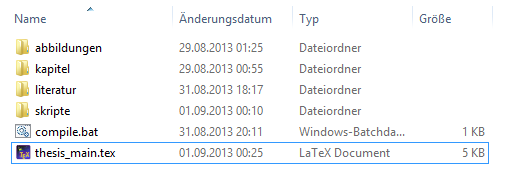
\includegraphics[width=0.9\textwidth]{verzeichnisStruktur}
\\
Quelle: Eigene Darstellung
\end{figure}
